%! Author = vladimir
%! Date = 3/1/23

% Preamble
\documentclass[12pt,a4paper]{article}

% Packages
\usepackage[slovak]{babel}
\usepackage[utf8]{inputenc}
\usepackage[T1]{fontenc}
\usepackage{float}
\usepackage{lmodern}
\usepackage[none]{hyphenat}
\usepackage[left=2cm, text={17cm, 24cm}, top=2cm]{geometry}
\usepackage{graphicx}
\usepackage{xcolor}
\usepackage{amsmath}
\usepackage{amssymb}
\usepackage{caption}
\usepackage{subcaption}
\usepackage{titlesec}
\usepackage{hyperref}
\usepackage{listings}
\usepackage{enumitem}
\usepackage{wasysym}
\usepackage{fancyhdr}
\usepackage{lastpage}
\usepackage{newpxtext}
\usepackage{longtable,ltcaption}
\usepackage{textgreek}
\usepackage{multirow}
\usepackage{outlines}

% \comment{}
\newcommand{\comment}[1]{}



% Document
\begin{document}

    % TITULNI STRANA
    \pagestyle{empty}
    \begin{titlepage}
        \begin{center}
            \normalsize{Vysoké učení technické v Brně\linebreak}
            \normalsize{Fakulta informačních technologií}

            \vfill

            \large\textbf{Databáze\linebreak}
            \large\textbf{2021/2022}

            \vfill

            \LARGE\textbf{Datový model (ERD) a model případů užití\linebreak}
            \large\textbf{Tým xzoban02}

            \vfill
            \vfill
            \vfill


            \begin{flushleft}
                \large
                Radek Zobaník (xzoban02)\\
                Vladimír Mečiar (xmecia00)
                \hfill
                Brno, \today
            \end{flushleft}
        \end{center}
    \end{titlepage}
    \pagestyle{plain}
    \newpage

    % CONTENT
    \section{Riešenia 4. úlohy}
    % Obrazek
\begin{figure}[h]
    \centering
    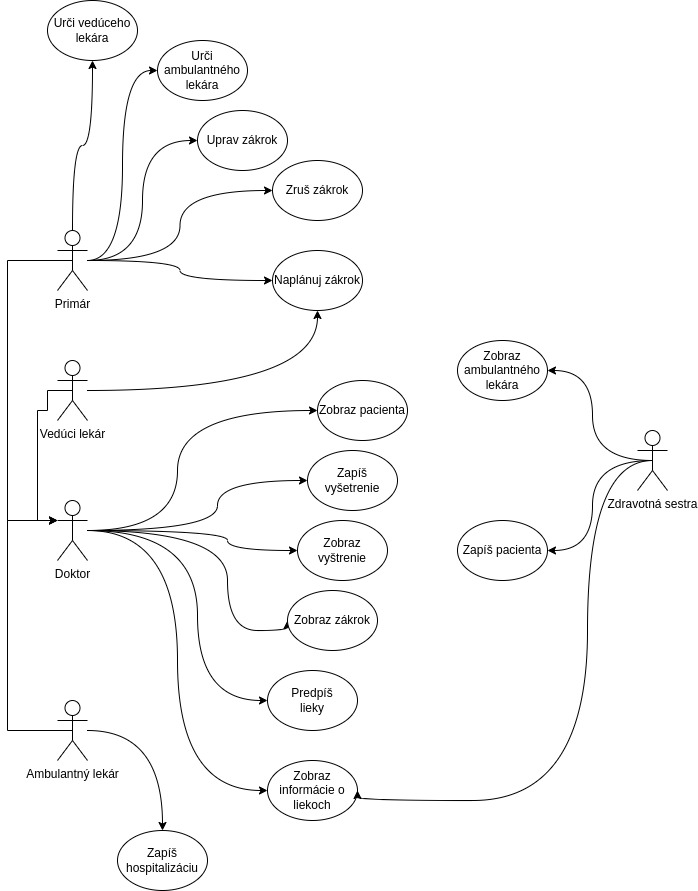
\includegraphics[width = \textwidth]{src/img/Nemocnica_use-case_Diagram.jpg}
    \caption{Model automatu}
    \label{fig:use_case}
\end{figure}

    % Obrazek
\begin{figure}[h]
    \centering
    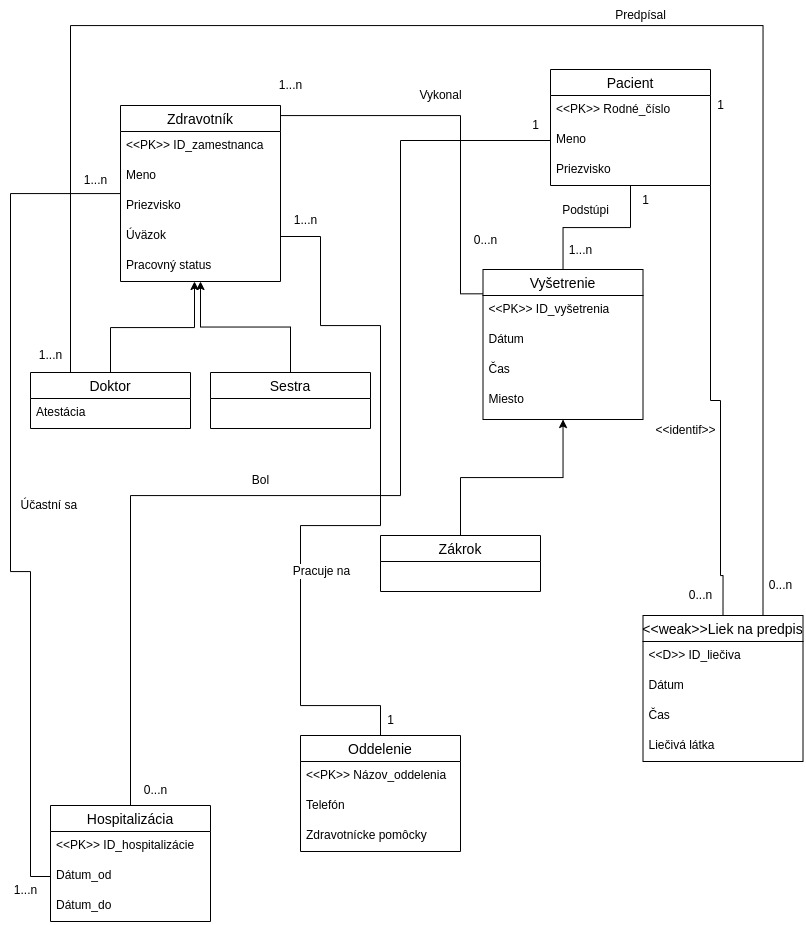
\includegraphics[width = \textwidth]{src/img/nemocnice_ER_DIAGRAM_1.jpg}
    \caption{Entity relationship diagram}
    \label{fig:er_diagram}
\end{figure}


\end{document}
